\documentclass[11pt]{report}

\usepackage[utf8]{inputenc} % Required for inputting international characters
\usepackage[T1]{fontenc} % Output font encoding for international characters
% \usepackage[demo]{graphicx} % images % get rid of [demo] for black box removal
\usepackage{graphicx} % images % get rid of [demo] for black box removal
\usepackage{fancyhdr} % headers and footers
\usepackage{parskip} % paragraph
\usepackage{geometry} % page size
% \usepackage{hyperref} % Links
% \usepackage{pdflscape} % making a page landscape
\usepackage{xcolor}
\usepackage[shortlabels]{enumitem}
\usepackage{multirow}
\usepackage{listings}
\usepackage{titlesec}
\usepackage{float} % to place figures in place
\usepackage{xurl}

% colors
\usepackage{xcolor}
\definecolor{mygrey}{RGB}{200, 200, 200}


% Helvetica as font
\usepackage[scaled]{helvet}
\renewcommand\familydefault{\sfdefault} 
% \usepackage[scaled=0.8]{FiraMono}

\graphicspath{{../images/}}

\titleformat{\chapter}[display]
  {\normalfont\bfseries}{}{0pt}{\Huge}

% margins and page size
\geometry{
a4paper,
left=30mm,
top=25mm,
right=30mm,
bottom=25mm
}

% \lstset{
%   basicstyle=\ttfamily,
%   columns=fullflexible,
%   frame=single,
%   breaklines=true,
%   postbreak=\mbox{\textcolor{red}{$\hookrightarrow$}\space},
% }

\definecolor{mygreen}{rgb}{0,0.6,0}
\definecolor{mygray}{rgb}{0.5,0.5,0.5}
\definecolor{mymauve}{rgb}{0.58,0,0.82}
% code formatting
\lstset{ %
  backgroundcolor=\color{white},   % choose the background color
  basicstyle=\ttfamily\footnotesize,    % fixed spaced font familyy  &  size of fonts used for the code
  breaklines=true,                 % automatic line breaking only at whitespace
  postbreak=\mbox{\textcolor{red}{$\hookrightarrow$}\space},
  captionpos=b,                    % sets the caption-position to bottom
  commentstyle=\color{mygreen},    % comment style
  escapeinside={\%*}{*)},          % if you want to add LaTeX within your code
  keywordstyle=\color{blue},       % keyword style
  stringstyle=\color{mymauve},     % string literal style
  frame=single,                    % border
}


\pagestyle{fancy}
\fancyhf{}
\rhead{Aum Patel}
\cfoot{\thepage}

% % in line code with bg command
% \newcommand{\code}[1][]{%
% \colorbox{mygrey}{\lstinline{#1}}%
% }

\begin{document}

%title
\author{Aum Patel - 180000492}
\title{Computer Graphics}
\maketitle

\section*{Overview}
The project I have created is based around a 'candy cane' style theme, where everything is vibrant and multi-coloured. The player has to collect all the points and can pick up speed power ups. 

\section*{Annotated Game Scene}

\begin{figure}[H]
    \begin{minipage}{.5\textwidth}
        \centering
        \fbox{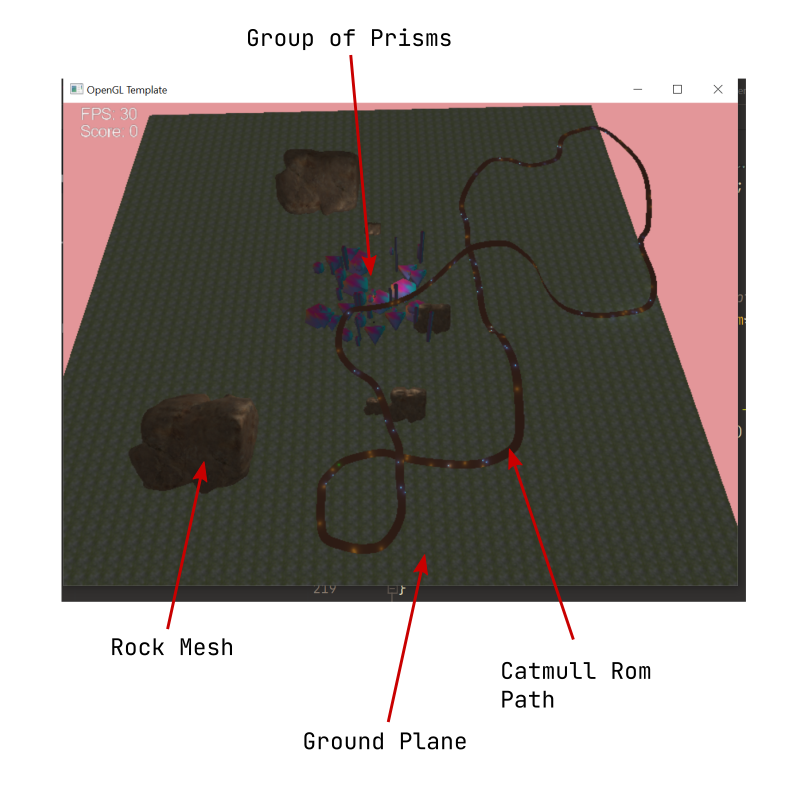
\includegraphics[width = 7cm ]{Zoomed Out Labelling.png}}
        \caption{Top Down view of the game scene, zoomed out}
    \end{minipage}
    \begin{minipage}{.5\textwidth}
        \centering
        \fbox{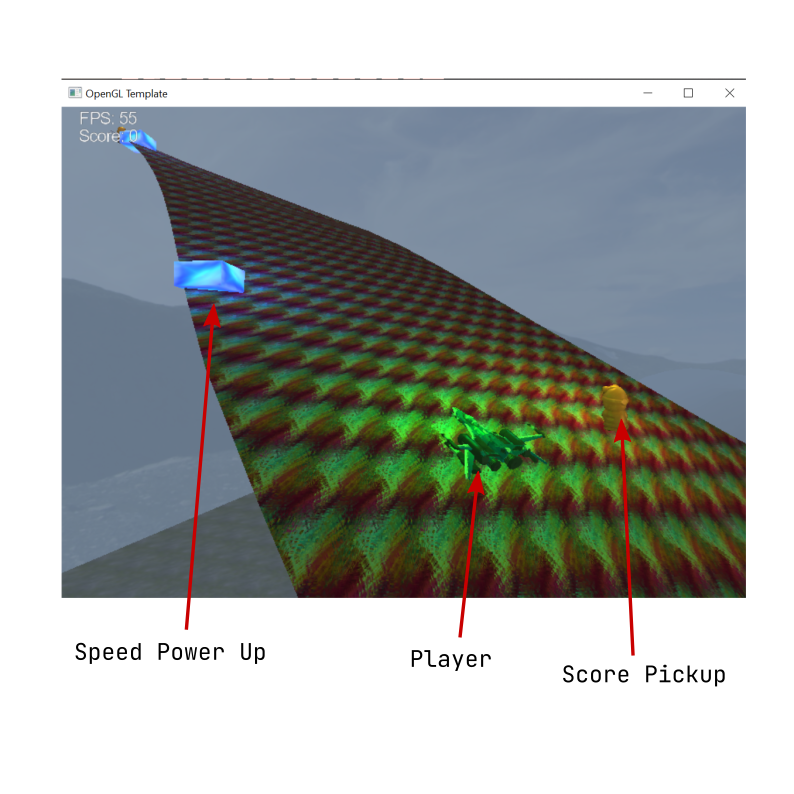
\includegraphics[width = 7cm ]{Player_Pickups_Zoomed_In.png}}
        \caption{Close view of the player, speed power-up and score power-up}
    \end{minipage}
\end{figure}

\section*{User Guide}
The goal of the game is to collect as many chocolate Santa Clause's as possible to get a high score. The player can pick up the blue pointed shape to gain a temporary speed boost.
    \begin{table}[H]
        \begin{center}
            \begin{tabular}{|l|l|}
            \hline
            \textbf{Controls}    & \textbf{Description}  \\
            \hline
              &  \\[0.5pt]
              Up Arrow    & Accelerate                   \\[10pt]
              Down Arrow  & Deccelerate                  \\[10pt]
              Left Arrow  & Move Left                    \\[10pt]
              Right Arrow & Move Right                   \\[10pt] 
              F           & Switch Camera View           \\[10pt]
              W A S D     & Camera Movement in Free Roam \\[10pt]
            \hline
            \end{tabular}
            \caption{Controls for the game}
        \end{center}
    \end{table}


\section*{Route and Camera}

% Route
\subsection*{Route}
% Planning
To plan out the path, Blender was used, as this provided an easier time visualising it over pen and paper. After sketching, I measured and listed the vertices out which are then used in the Catmull Rom \colorbox{mygrey}{\lstinline{SetControlPoints()}} method; the measurement displayed in the image below are rounded to the nearest fifth, as the Blender measure tool does not snap. 
\begin{figure}[H]
    \centering
    \fbox{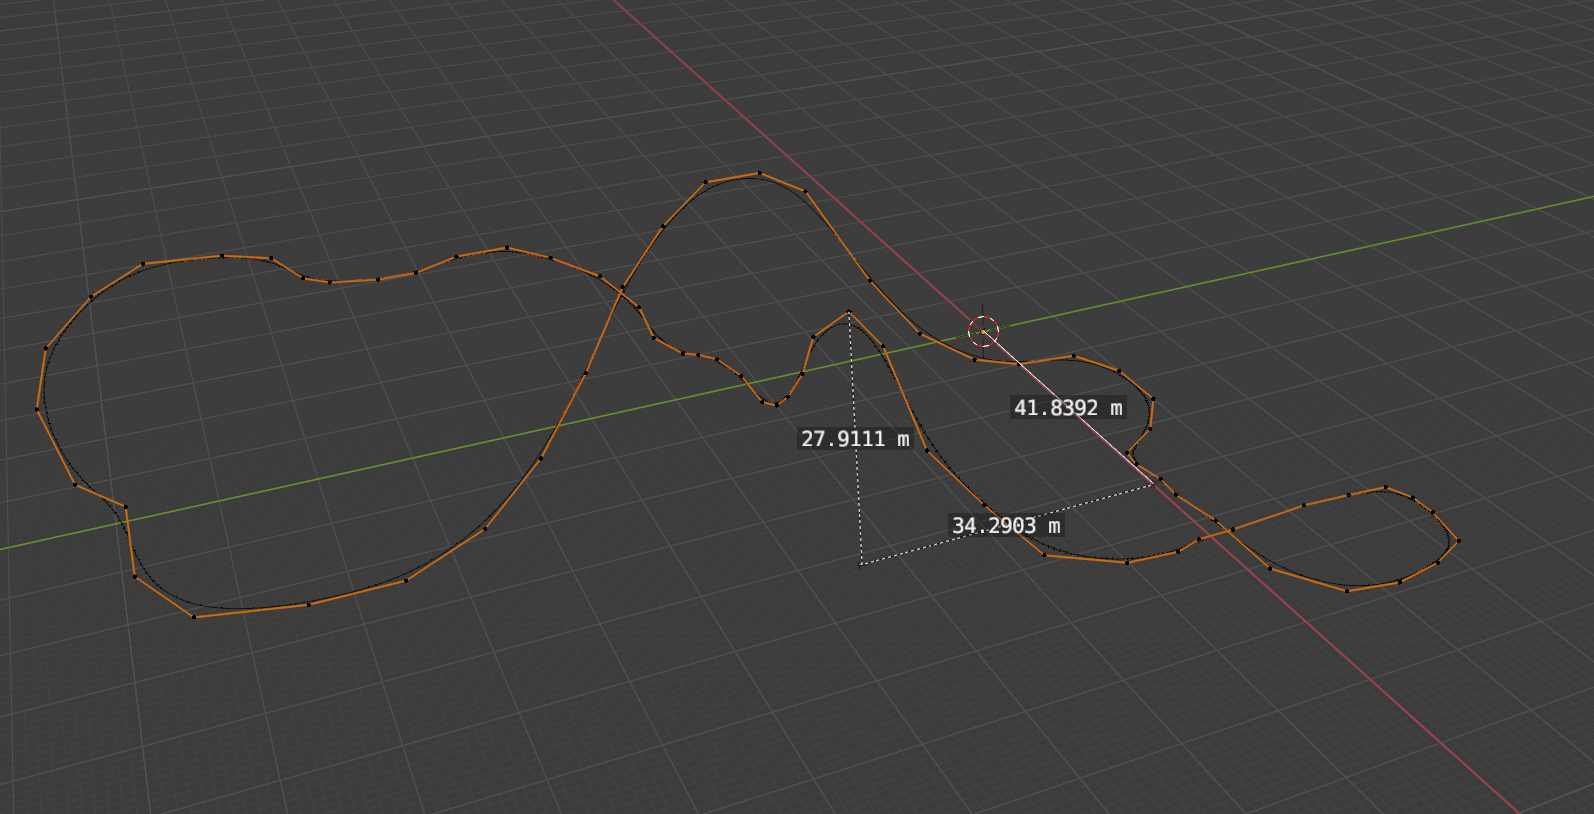
\includegraphics[width = 14cm]{Path_Plan_in_Blender.png}}
    \caption{Path Sketched out in Blender}
\end{figure}

% Adding Control Points
When adding the points into the \colorbox{mygrey}{\lstinline{SetControlPoints()}} method, I decided to create some parameters and add/multiply those to the vertices I was adding in, these parameters were a scalar value on the xyz axis and an offset value on the xyz (which is multiplied by the scalar before being applied to the control points). This way I could move the path around freely without needing to adjust the vertices.


% \begin{lstlisting}[language=c]
% SetControlPoints(){
%     // parameters to adjust the scaling and positioning of the path.
%     const float xScale = 10.f;
%     const float zScale = 10.f;
%     const float yScale = 10.f;
%     const float xOffset = 0 * xScale;
%     const float zOffset = 0 * zScale;
%     const float yOffset = 10 * yScale;

%     // example for one control point. Total of 70 points
%     m_controlPoints.emplace_back(xOffset + xScale * 59.0, yOffset + yScale * 5.0, zOffset + zScale * 7.0);
% }
% \end{lstlisting}

\subsection*{Camera}
I have implemented 5 camera modes: \textbf{First Person}, \textbf{Third Person}, \textbf{Left Side View}, \textbf{Right Side View} and \textbf{Top View}.

% Switching Camera modes
I switch between them by storing the current \colorbox{mygrey}{\lstinline{cameraType}} as an integer, and have a set of camera modes:
\begin{lstlisting}[language=c]
    static const glm::uint FIRST_PERSON = 0;
    static const glm::uint THIRD_PERSON = 1;
    ... // and so on
\end{lstlisting}
When switching camera mode, I change the camera type and check against this set of constant integers when setting the view of the camera by the spline and place the camera relative to the path with different distance values.

% First Person Camera Mode
I generate a TNB frame in every instance and offset the camera's position relative to the TNB frame to move it along local coordinates. For the \textbf{first person view} I moved it up one value on the bi-normal to place it just above the nose of the spaceship.

For the \textbf{3rd person view}, I moved it even higher and placed it slightly behind the car so the whole track can be seen. When in the 3rd person view, the camera does not follow the left and right movement of the car like it does in First Person.

For the \textbf{side views} I multiply a positive/negative (for both left/right sides) offset value by the normal and place the camera's 'look at' at the car's position.

Similar to the \textbf{top view}, moving it up on the binormal and having the camera look down at the car.

As well as these views, I still have the free view available to toggle to make it easy to debug.

\newpage
%=============
% 3
%=============
\section*{Basic Objects, Meshes and Lighting}
A game object class was created to easily create more shapes and contain shared behaviours.

\subsection*{Basic Objects}
I have two shapes that I have created using primitives: a house type shape, that is laid on the side to represent an arrow for a speed power-up; and a prism shape for which different parameters can be passed through to generate all different types of prisms. 

\subsubsection*{House Shape}
For this shape, I implemented a class for the house style shape that we planned out in the interim submission. This shape can be found in \colorbox{mygrey}{\lstinline{mSpeedPowerUp.h/cpp}}. I used \colorbox{mygrey}{\lstinline{GL_TRIANGLES}} to render the shape as this is how I sketched the drawing on paper. This creation of this shape can be modified by 3 parameters, \lstinline{length, width, height}, this allows for repurposing the shape in the future.

This shape is textured and a light is placed in its location.
\begin{figure}[H]
    \centering
    \fbox{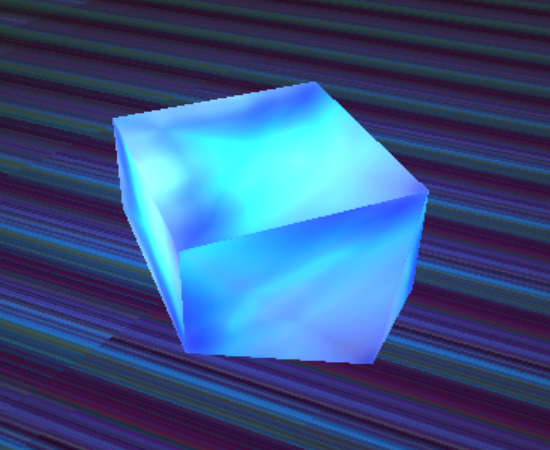
\includegraphics[width = 7cm]{Primitive_House.png}}
    \caption{Speed Power up in Game}
\end{figure}

\subsubsection*{Prism}
For the prism shape, I wanted to create it so that I can provide it \lstinline{radius, height, side_count} and create a shape with it. To understand the maths behind creating a prism, a tutorial was used \footnote{Song Ho, OpenGL Cylinder, Prism \& Pipe : \url{http://www.songho.ca/opengl/gl_cylinder.html}}; I calculate the vertices on the \textbf{base} of the prism and the \textbf{top} of the prism (which is the same as the base, just offset by height and in reverse order); I then take both of these, alternate between them to create a set of \textbf{side vertices}. With both the top and base I render them using \lstinline{GL_TRIANGLE_FAN} as I require only a minimal number of vertices to store, I require a centre plus the number of sides; I then use a \lstinline{GL_TRIANGLE_STRIP} between the side vertices to get all triangles rendered facing outside appropriately.

I create multiple prisms and pass the parameters by parsing string, e.g.\\ \colorbox{mygrey}{\lstinline{prismsToGenerate.push_back("r5h20s3");}} will add a prism to be created with a radius of 5, height of 20 and a side count of 3. 

After generating a small number of varying prisms, I generate a number of random position to place the prisms in-game. As well as position, I have 2 other vectors representing the prisms to be placed in the scene, this being the random scale (providing extra variety to the shapes), and the index of the specific prism VAO to use. In the render method, the position vector is iterated through and the appropriate prisms are rendered in their correct locations.

These prisms are currently used as scenery and have a nice colourful texture on them. 
\begin{figure}[H]
    \centering
    \fbox{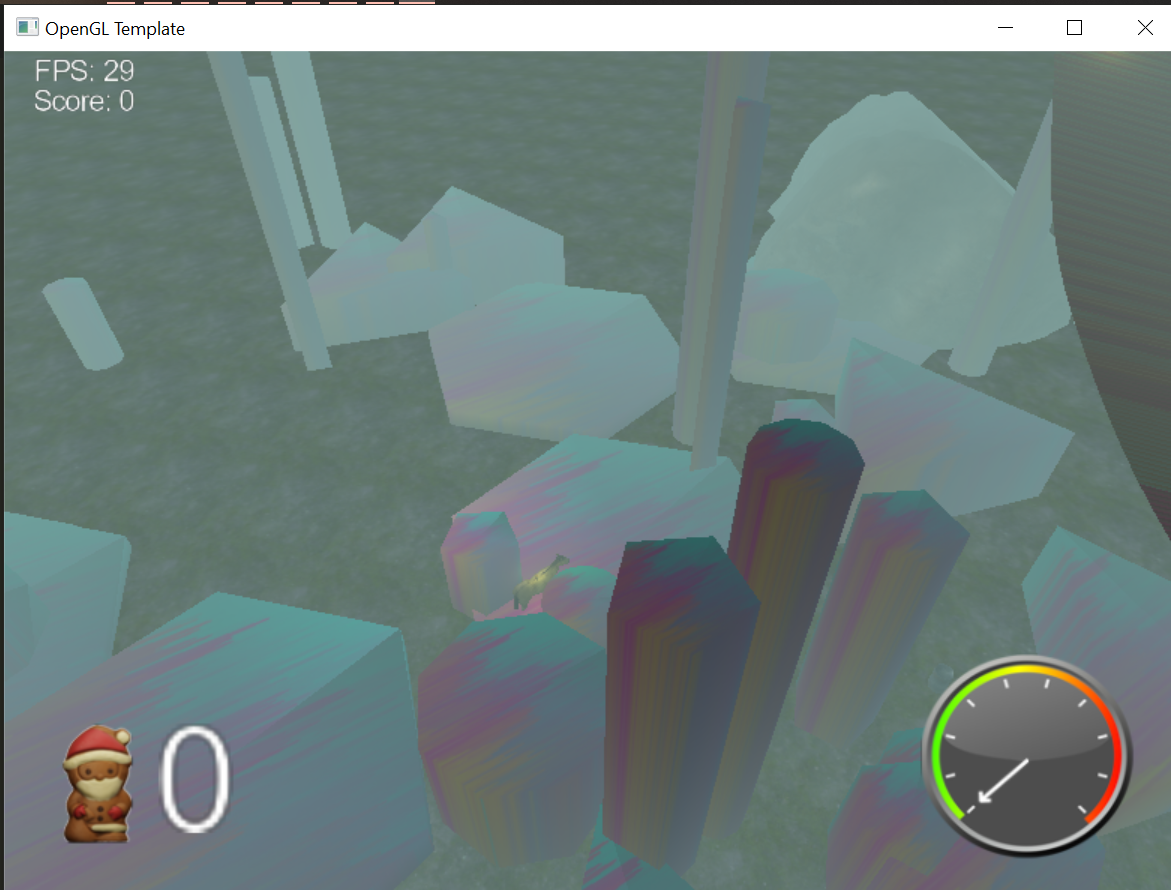
\includegraphics[width = 10cm]{Shapes_Prisms.png}}
    \caption{Prisms in scene}
\end{figure}

\subsubsection*{Meshes}
I have loaded 3 meshes into the scene, the player's spaceship, the chocolate Santa Clauses, and the rocks that make up the scenery.

These meshes have been loaded up as meshes inheriting the GameObject class. Only one instance of the mesh is rendered, and then the mesh is 

\begin{figure}[H]
    \begin{minipage}{.5\textwidth}
        \centering
        \fbox{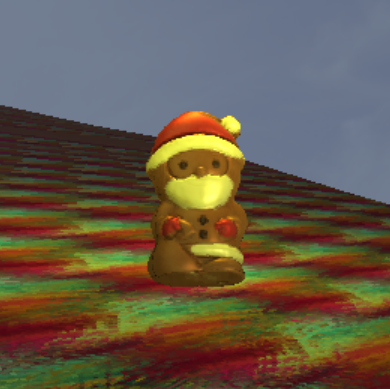
\includegraphics[width = 7cm ]{Choco_Santa.png}}
        \caption{Chocolate Santa Clause mesh}
    \end{minipage}
    \begin{minipage}{.5\textwidth}
        \centering
        \fbox{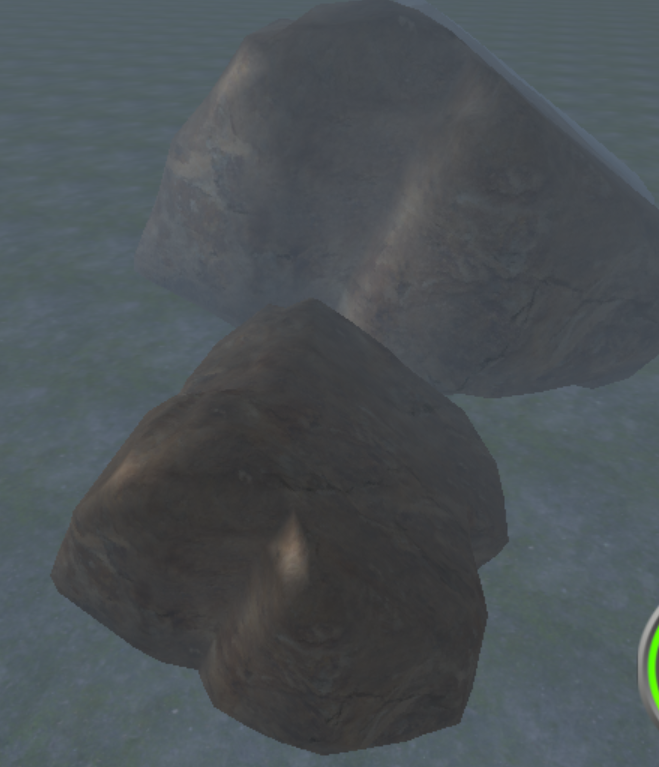
\includegraphics[width = 7cm ]{Rocks.png}}
        \caption{Rock mesh}
    \end{minipage}
\end{figure}

\begin{figure}[H]
    \centering
    \fbox{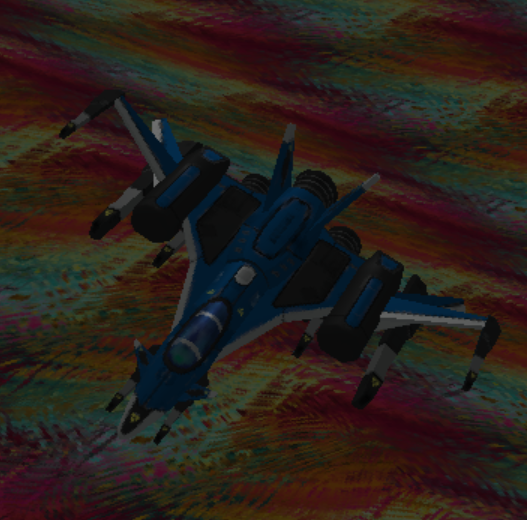
\includegraphics[width = 7cm]{Player_Ship.png}}
    \caption{Player Space Ship (with point light off)}
\end{figure}

\subsection*{Lights}
% TODO check figure numbers
Multiple dynamic point lights were added into the scene, there is one point light on every pickup\footnote{These point lights are also dynamic however the pickups only move up and down.} (Fig 4, 6), of different colour, and there is a point light on the player's ship. The point light on the player's ship moves around with the player.

These point lights have been added by creating a Phong model that is point light specific \footnote{Lecture 6 and the Phong model in the mainShader.vert used as reference} inside the fragment shader; a point light is defined by a structure that contains the information required to render a light appropriately.
\begin{figure}[H]
    \centering
    \fbox{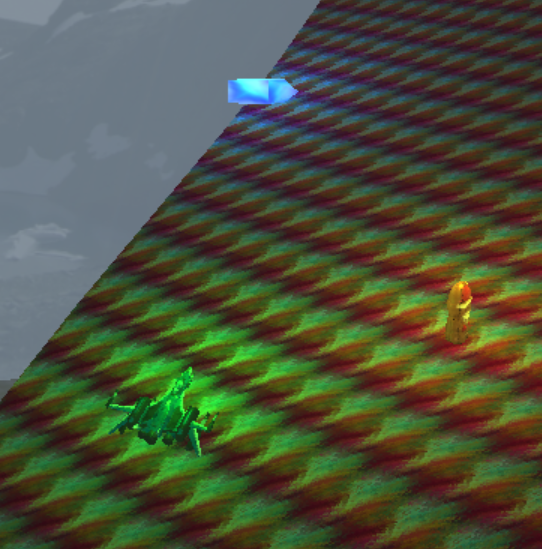
\includegraphics[width = 10cm]{Point_Lights.png}}
    \caption{Examples for Point lights}
\end{figure}

For the many point lights in the scene, I created an array of a fixed size of 100, so it is flexible in that I can add more lights without resizing the array at runtime.

\newpage
%=============
% 4
%=============
\section*{HUD, Gameplay and Advanced Rendering}
\subsection*{HUD}
To create the HUD, I chose to use full-screen PNG's that act as sprites in the game and are rendered on top of the rendered frame using a full-screen quad. I created a \colorbox{mygrey}{\lstinline{HudItem}} class which holds one or multiple textures and can be 'bound' to the renderer by passing in an index to the texture wanting to be rendered; these textures are stored inside a vector. The \colorbox{mygrey}{\lstinline{HudManager}} will then render the many HudItems that are created.

% \begin{lstlisting}[language=c]
% void HudManager::Create() {
%     ...
%     // create a full screen quad
%     ...
%     Santa.AddTexture("resources\\textures\\hud\\Santa_png\\Santa.png");

%     for (int i = 1; i <= 6; ++i) {
%         speedometer.AddTexture("resources\\textures\\hud\\speedometer_png\\speed_" + to_string(i) + ".png");
%     }
%     speedometer.AddTexture("resources\\textures\\hud\\speedometer_png\\speed_boost.png");
% }

% void HudManager::Render(CShaderProgram* shader) {
%     // Draw Santa
%     glBindVertexArray(quadVAO);
%     Santa.Bind(0);
%     glDrawArrays(GL_TRIANGLES, 0, 6);

%     // Draw Speedometer
%     glBindVertexArray(quadVAO);
%     // will draw the appropriate speedometer texture
%     speedometer.Bind(speedometerIndex);
%     glDrawArrays(GL_TRIANGLES, 0, 6);
% }
% \end{lstlisting}

Below are figures that show how the different hud items are displayed.
\begin{figure}[H]
    \begin{minipage}{.5\textwidth}
        \centering
        \fbox{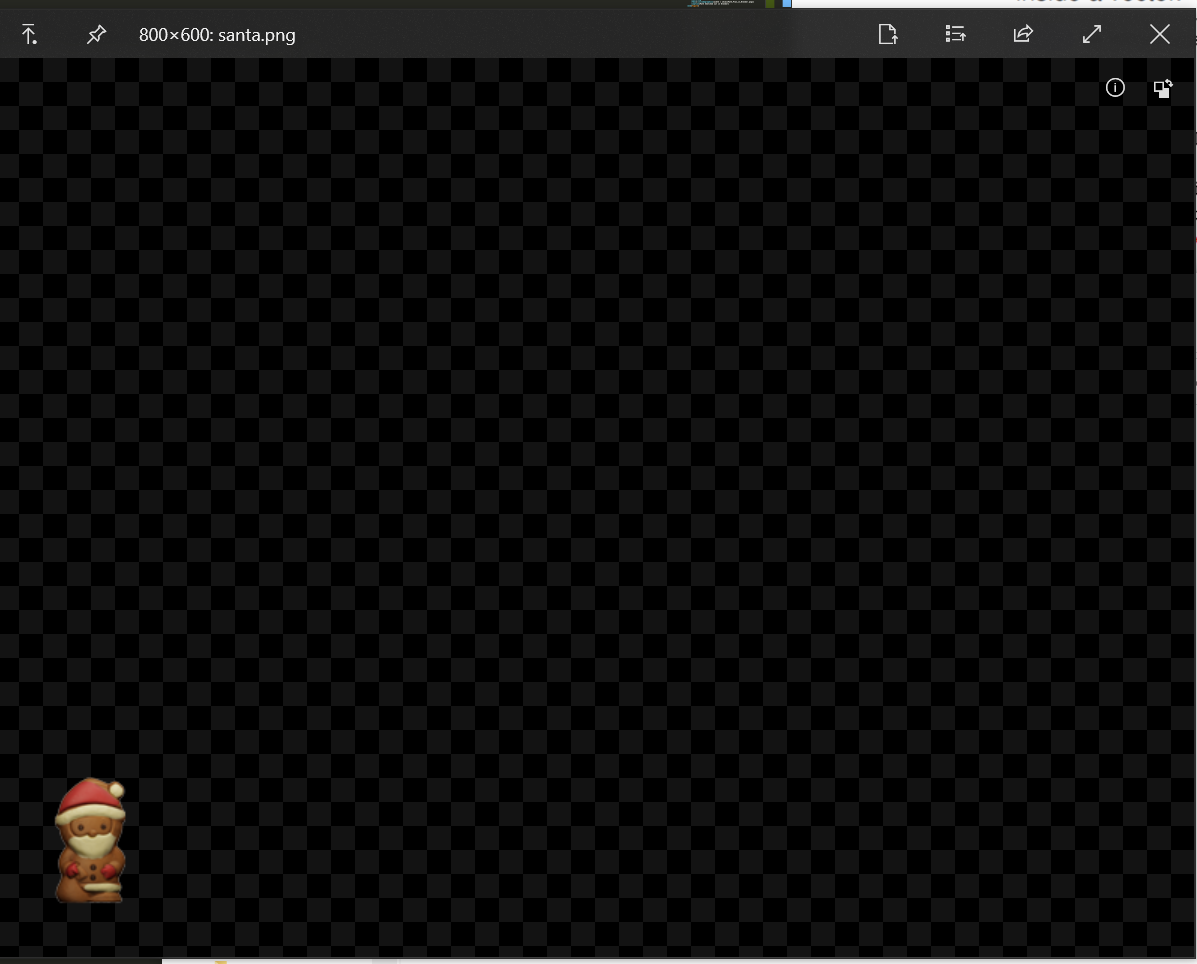
\includegraphics[width = 7cm ]{HUD_Santa.png}}
        \caption{Score HUD Item}
    \end{minipage}
    \begin{minipage}{.5\textwidth}
        \centering
        \fbox{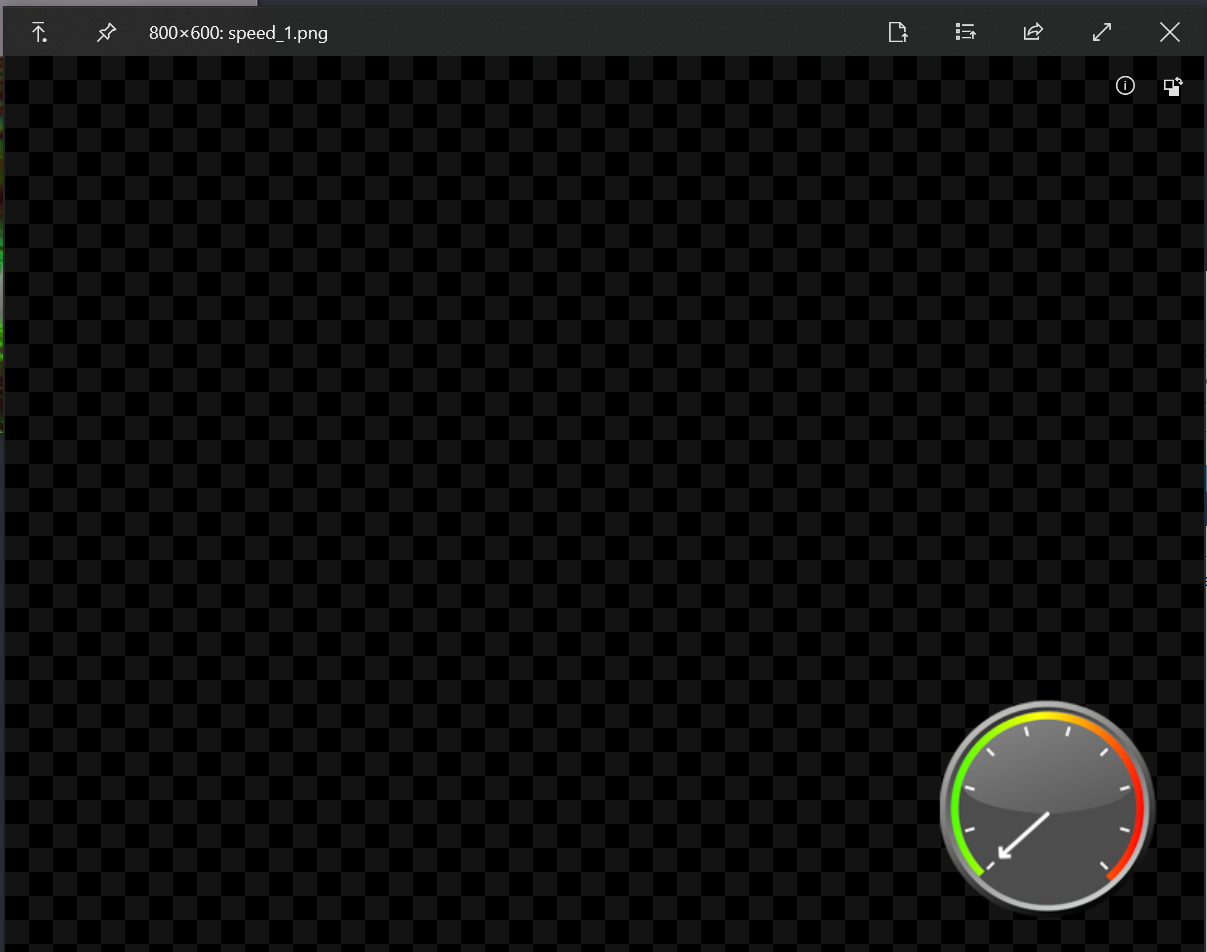
\includegraphics[width = 7cm ]{HUD_Speedometer.png}}
        \caption{Speedometer Hud Item}
    \end{minipage}
\end{figure}

\begin{figure}[H]
    \centering
    \fbox{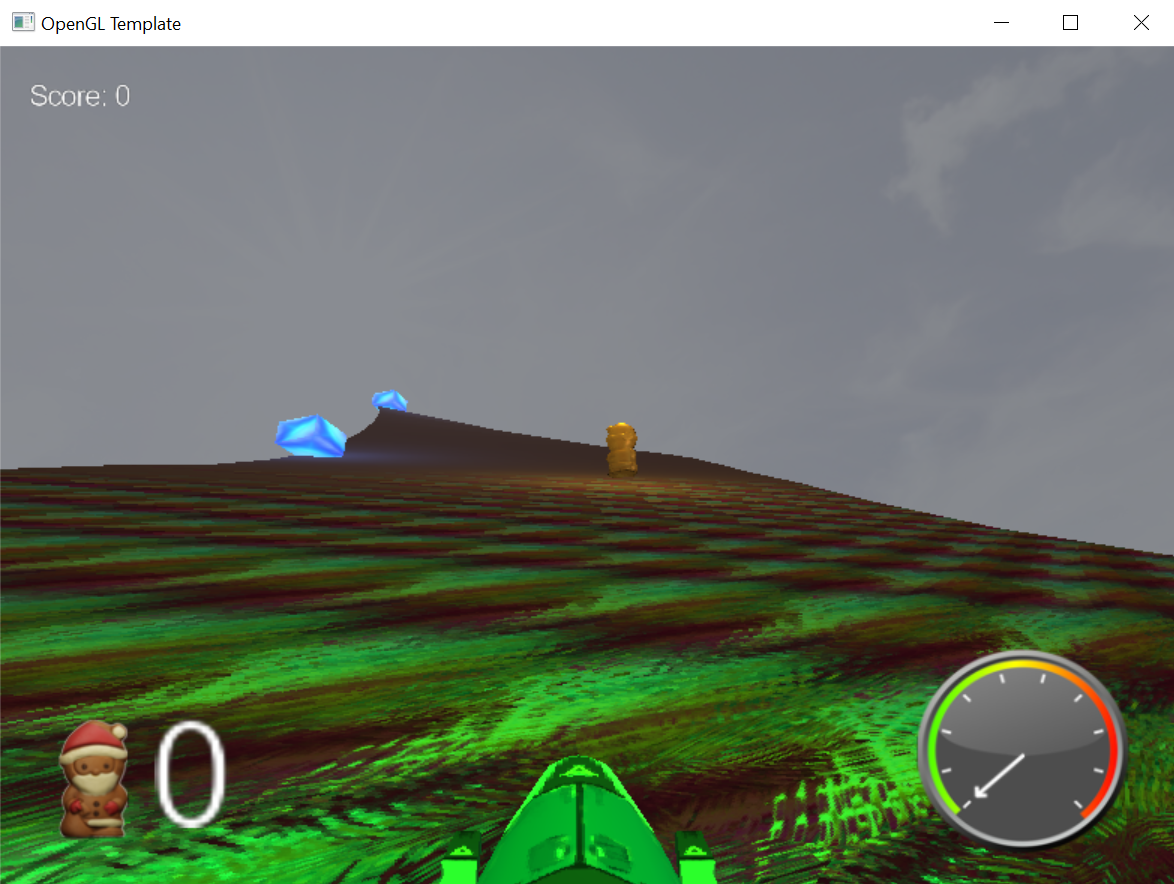
\includegraphics[width = 10cm]{Hud_In_Game.png}}
    \caption{Hud as Displayed in Game}
\end{figure}

As I can store multiple textures within one HudItem, I have stored 7 different images for the speedometer, and based on the speed of the player, I switch between 6 of them and change to the 7th one when they pick up the speed powerup. This creates an interactive HUD.

As well as the two HUD classes that I created, I also needed a shader to render the 2D elements appropriately. This is a very basic shader that maps the texture's colour to the fragment shader. This is all then rendered after the radial blur in the main Game \colorbox{mygrey}{\lstinline{Render()}} method. This shader was created by taking the radial blur shader, which was already a 2d shader, and removing the values that created the blur effect, essentially giving me a simple 2d shader.

When rendering multiple full-screen elements, the \colorbox{mygrey}{\lstinline{GL_DEPTH_TEST}} had to be disabled, otherwise, only the first element rendered will show; disabling depth test is done to avoid 'plane fighting' where two overlapping faces will clash with each other, however, for the HUD, rendering multiple quads on the same 'plane' needed this to be disabled, to have all elements rendered.

\subsection*{Gameplay}
\subsubsection*{Control}
By pressing the upwards arrow key, the car will accelerate until it reaches the max limit, and vice versa when pressing the down arrow key; when the key is released, the speed will be kept unchanged. This is done by creating a speed value and setting it in both the \textbf{Car} and \textbf{Camera} objects, and changing the value that is being set on the appropriate key presses.

When pressing the Left and Right Arrow keys, the car placed on an offset from the centre of the Catmull Rom path. This offset is applied via the TNB frame on the Normal of the car and the camera (only applied to the camera when in First Person View).
\begin{lstlisting}[language=c]
    mPlayerXOffset -= m_dt * mCar->getXOffsetSpeed(); // + for moving right
    mCar->setXOffset(mPlayerXOffset);
    m_pCamera->setXOffset(mCar->getXOffset());
\end{lstlisting}

\subsubsection*{Collision Detection}
The collision detection used in the game is very simple, however is made easier by using a generalised \colorbox{mygrey}{\lstinline{GameObject}} class, this class contains the collision radius of an object. Any object that is rendered on screen is a child of GameObject. Every frame in the \colorbox{mygrey}{\lstinline{Update()}} loop of my game, I call a function \colorbox{mygrey}{\lstinline{ManageCollisions()}}, which traverses the many vector's that store the positions to render the different game objects and calls \\ \colorbox{mygrey}{\lstinline{CheckCollision(aPos, aRadius, bPos, bRadius)}} that compares the radius between two objects and returns true if they overlap.

When a collision happens, I store the iterator/position inside of the vector of positions and remove it; On doing so, the object in that position will stop rendering, simulating the player picking it up.

\subsubsection*{Gameplay Elements}
Depending on which object it collides with, a different behaviour occurs. For the score pickup, the player's score is incremented by 1, and if it is the speed power-up, then \colorbox{mygrey}{\lstinline{mSpeedPowerUpTimer}} is set to 1 second, which makes a boost activate. The player just needs to pick up as much chocolate as they can. If they pick up all the points, a game over message will display.
\begin{figure}[H]
    \centering
    \fbox{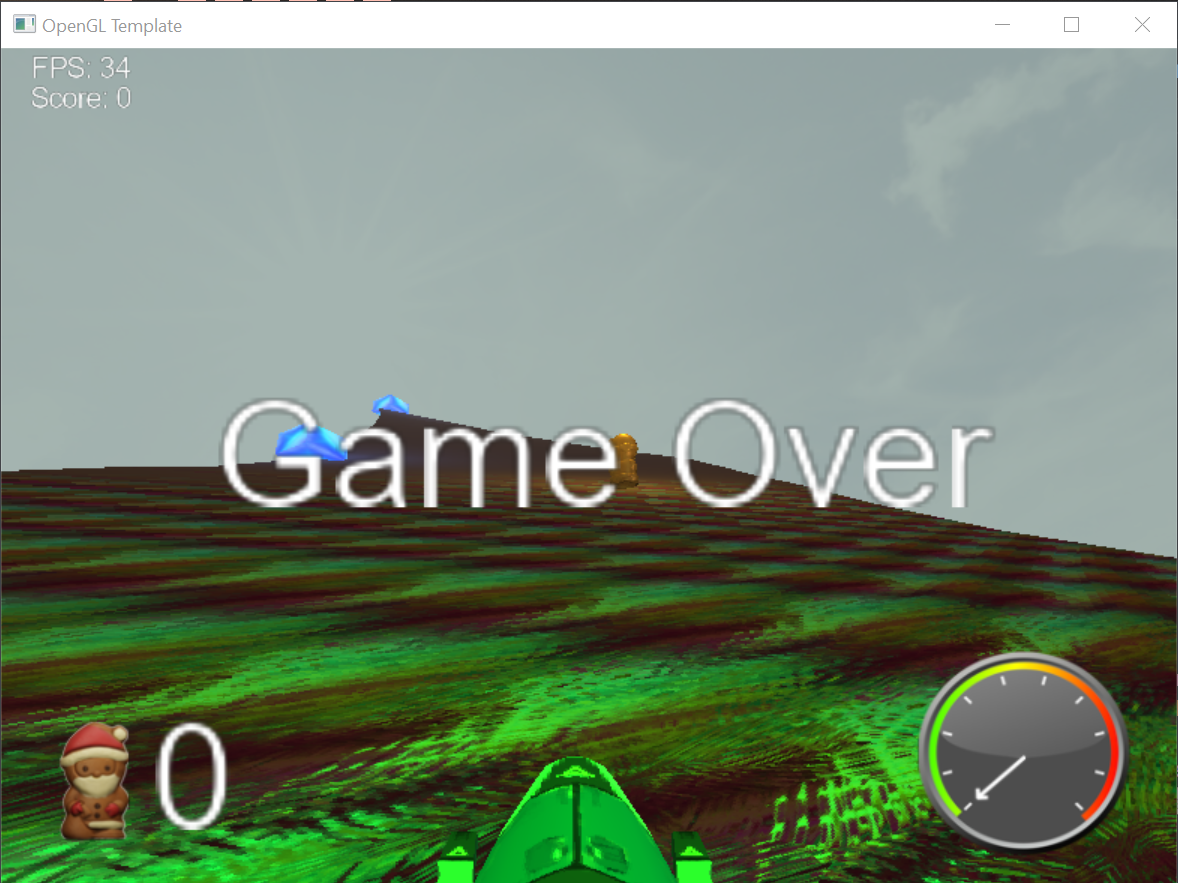
\includegraphics[width = 10cm]{Game_Over_Screen.png}}
    \caption{Game Over Screen}
\end{figure}

\subsection*{Advanced Rendering}

\subsubsection*{Fog}
Two advanced rendering techniques were implemented, the first one was fog. This was achieved by following a tutorial \footnote{Tutorial by Thin Matrix for Fog in OpenGL \url{https://youtu.be/qslBNLeSPUc}}. This tutorial described the shader that had to be created, I followed this and adjusted the parameters to get fog that displayed correctly; the \colorbox{mygrey}{\lstinline{mainShader.vert/frag}} was changed to add the fog. As the distance from the player to the object is calculated in the vertex shader per vertex, the distance for large objects, such as the terrain and skybox, is not presented correctly. To rectify this, the density and gradient for both terrain and skybox were lowered to make them visible. 

\begin{figure}[H]
    \centering
    \fbox{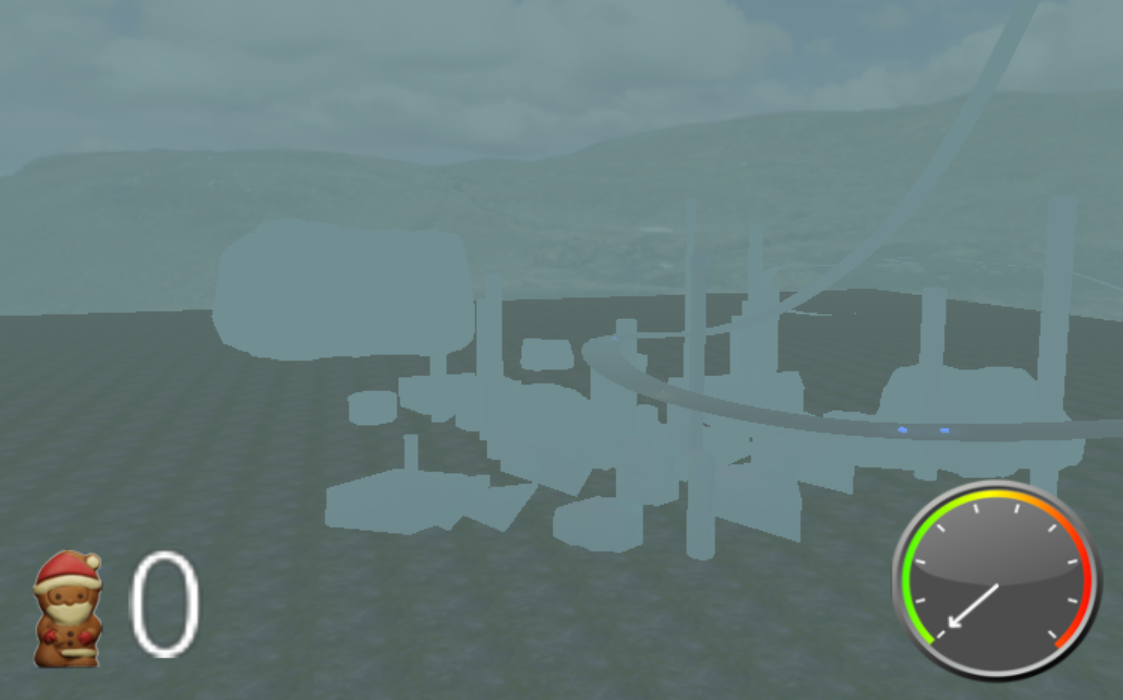
\includegraphics[width = 10cm]{Fog.png}}
    \caption{Fog in game scene}
\end{figure}

To add to the 'candyland' style theme of the game, the colour of the fog was randomly adjusted on the client side, and passed through to fragment shader as the sky colour, giving a nice vibrant ambience.

\subsubsection*{Radial Blur}
There is a radial blur that activates when a boost speed power-up is picked up noting to the player that they have sped up.

The radial blur was achieved by creating a separate shader files (\colorbox{mygrey}{\lstinline{radialBlur.vert/frag}}) for it. These shaders were created by following the tutorial provided in lecture 7 \footnote{INM376\_2021.L07.pdf, page 55 \url{https://stackoverflow.com/questions/4579020/how-do-i-use-a-glsl-shader-to-apply-a-radial-blur-to-an-entire-scene}}. As this tutorial/post was 10 years old, the shader code had to be ported over to version 400. The fragment shader takes 10 samples and distorts the texture that is passed through and set as the frag colour.

To get the rendered image as a texture, I had to create a \textbf{Frame Buffer Object}, the helper classes provided by the University were used to achieve this. I then render the scene in two passes; after the second pass is when any post-processing effect, like the radial blur. While using the shader, the texture of the previous frame is stored onto the FBO and is bound to the buffer, then the quad is rendered, displaying the radial blur. The radial blur only lasts the duration of speed boost power-up.
\begin{figure}[H]
    \centering
    \fbox{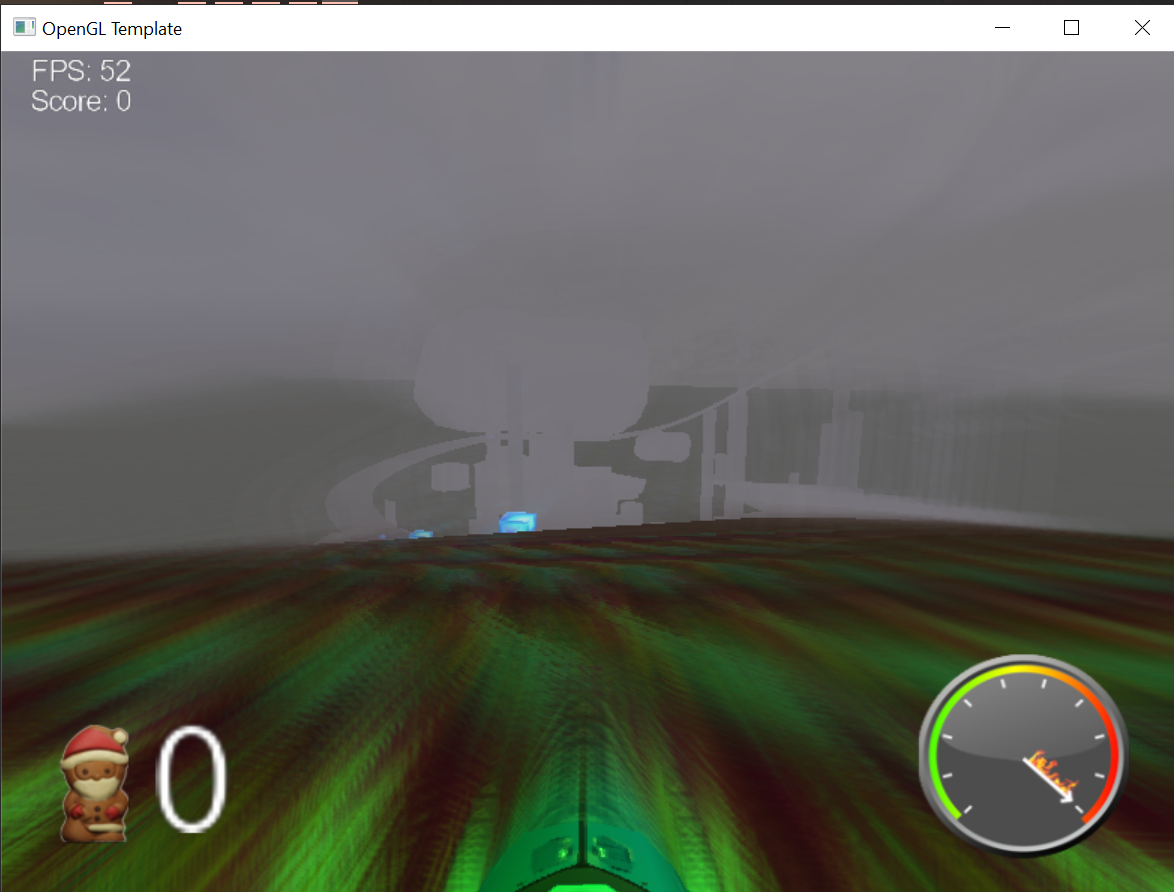
\includegraphics[width = 15cm]{Radial_Blur.png}}
    \caption{Radial Blur as seen in game}
\end{figure}

\newpage
%=============
% 5
%=============
\section*{Conclusion}
I am proud of what I have learnt about rendering computer graphics on screen and have come to appreciate more how much effort goes into optimising the program to squeeze as many frames as possible every second.

I like that there is somewhat of a goal for the player to work towards when playing the game, which is to collect all the points, however, I think player engagement would be greatly increased if there were some type of obstacles in the game; the game could be that they have to collect as many points as they can without touching any obstacles, adding extra challenge and increasing the replay value.

I am really happy that I got a working HUD that can display images, and change images based on code, like in the speedometer, which changes based on speed. I would like to take this a step further by adding more animated HUD elements onto the screen, with more fine-tune control.

The current point lights are nice, however, I think the one on the player is too intense. If there was more time, multi-coloured spotlights would be added to the game that move around on the track and adds an extra element to the candyland theme.

As nice as it is currently to move the player left and right along the track, some more animations to the player ship model would be a really nice addition.

Instance rendering is something I did not have time to attempt implementing, I could use instanced rendering to render the many prisms in the scenery, and that would increase the performance of the game greatly, as there would only be one draw call per type of prism. This instance rendering could also be expanded upon the pickups as there is no reason to not have them be instance rendered.

\newpage
\section*{Asset Listing}
\subsection*{Sky Box}
Emil Persson, aka Humus.

\url{http://www.humus.name}

This work is licensed under a Creative Commons Attribution 3.0 Unported License.

\url{http://creativecommons.org/licenses/by/3.0/}

\subsection*{Chocolate Santa Clause}
3D Choco Santa Claus 6 modelby 3dfood

\url{https://www.turbosquid.com/3d-models/3d-Santa-claus-model-1478073}

The TurboSquid 3D Model License

\subsection*{Player Ship}
spaceship 01 by ABDE “ESFEP”

\url{https://poly.google.com/view/aI32MU8lhd4}

CC-BY licence
\url{https://creativecommons.org/licenses/by/4.0/}

\subsection*{Rock}
free rock 3D modelby ice kazim

\url{https://www.turbosquid.com/3d-models/rock-3d-model-1577455}

The TurboSquid 3D Model License

\subsection*{Code}
Any reference to code is made in line in the code and in foot notes throughout this document.


\end{document}